\section{Background}

Flood reporting is a practical information problem before it becomes a software problem. A person near a flooded road may know what is happening before any official record is created, but that first message is often incomplete. It may include a photo but no ward name, a description but no coordinates, or a location pin without enough context to judge the situation. VietFlood is built around this gap. The system tries to turn quick local observations into structured reports that can be stored, searched, and reviewed later. This direction is consistent with the use of volunteered and citizen-generated information in crisis response, where local observations become more useful when they are organized for processing \cite{goodchild2010crowdsourcing,imran2015processing}.

The project does not aim to replace forecasting systems, hydrological models, or official emergency command centers. Its role is narrower and more concrete. VietFlood supports report submission from a mobile device, evidence upload, report storage, status tracking, relief awareness screens, and administrator review through a web dashboard. This scope is important because a flood management platform can become very broad. The thesis focuses on the part that was designed and implemented: moving field information from a citizen report into a backend record that an authorized user can inspect.

\subsection{Flood Reports as Structured Field Records}

An informal flood message can be fast, but it is not always easy to reuse. A chat message may be buried after a few minutes. A photo may be forwarded without its original location. A phone call may help one person but leave no shared record for others. VietFlood treats each citizen submission as a structured field record instead of a loose message.

The report entity in VietFlood stores the category, description, image links, evidence metadata, province, ward, address line, latitude, longitude, urgency flag, severity value, status, timestamps, and the account that created the report. These fields answer the questions that usually come first during review: what happened, where it happened, who reported it, how serious it appears, and what evidence supports the report.

The report status model is intentionally small. A report can be \texttt{pending}, \texttt{verified}, \texttt{resolved}, or \texttt{rejected}. A new submission begins as pending. An administrator can mark it as verified when the information is considered reliable, resolved when the case is no longer active, or rejected when the report is unsuitable or incorrect. Keeping rejected reports separate is useful because it preserves an audit trail instead of simply deleting every bad report.

\subsection{The Role of Mobile Reporting}

Mobile reporting is central to VietFlood because most observations are made away from a desk. A citizen may be standing near a flooded street, using a phone connection, and trying to submit a report quickly. For that reason, the citizen and relief-side application is built with Expo React Native \cite{expoDocs,reactNativeDocs}. The same mobile codebase supports authentication, profile pages, report creation, image selection, report lists, relief-oriented screens, maps, and role-aware navigation.

\begin{figure}[htbp]
    \centering
    \IfFileExists{images/figure2-1-report-lifecycle.png}{
        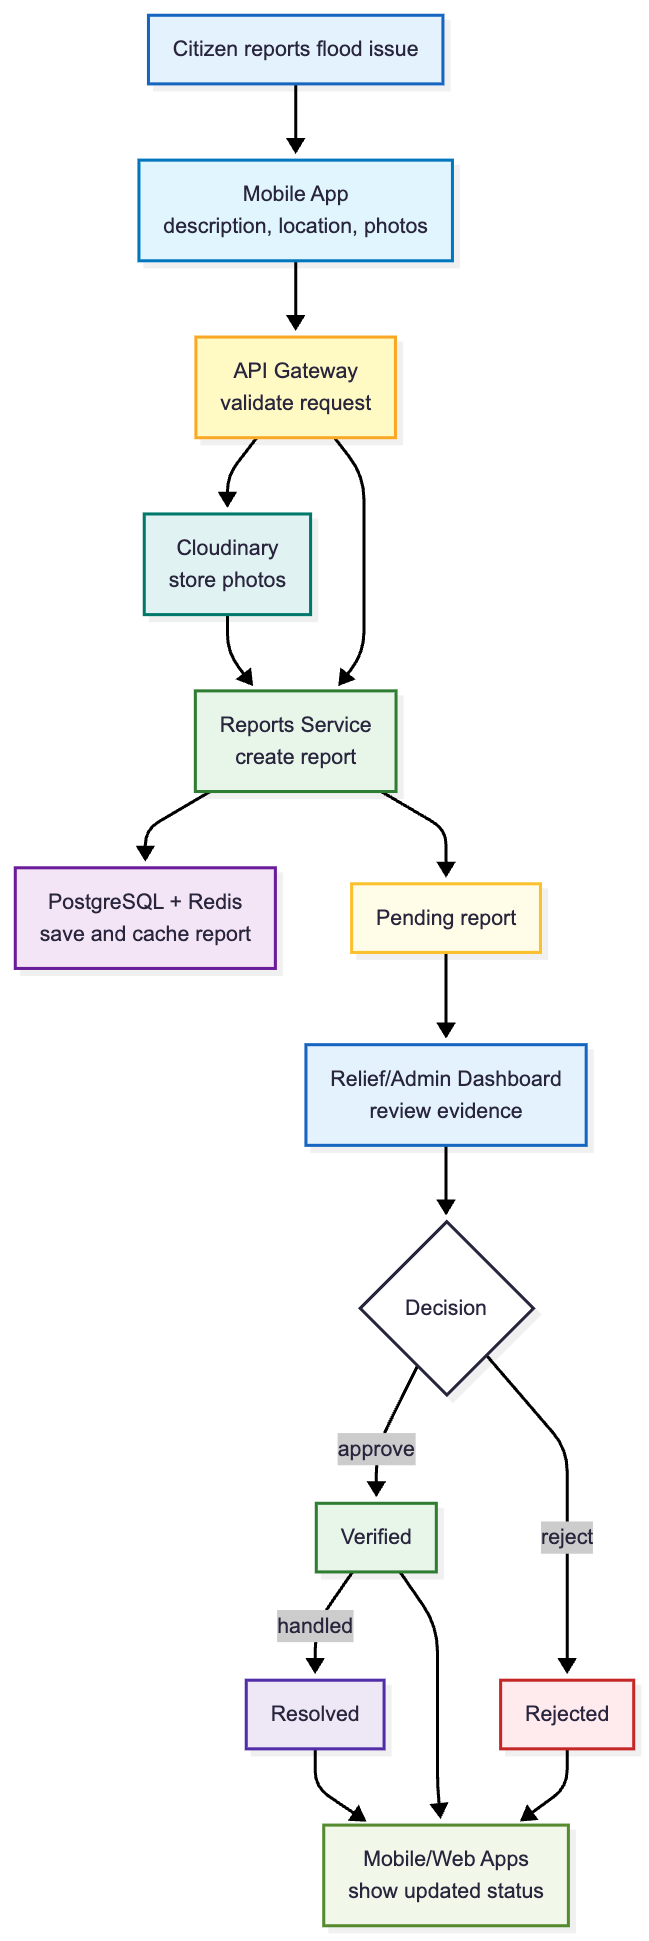
\includegraphics[width=1\linewidth,height=0.9\textheight,keepaspectratio]{images/figure2-1-report-lifecycle.png}
    }{
        \fbox{
            \begin{minipage}[c][4.8cm][c]{0.86\linewidth}
                \centering
                Placeholder for Figure 2.1\\[0.4cm]
                Suggested image: citizen creates report, gateway receives it, reports service stores it, reviewer changes status, dashboard shows updated case.\\[0.3cm]
                File name: \texttt{images/figure2-1-report-lifecycle.png}
            \end{minipage}
        }
    }
    \caption{Lifecycle of a VietFlood citizen report from mobile submission to review status.}
    \label{fig:chapter2-report-lifecycle}
\end{figure}

Figure~\ref{fig:chapter2-report-lifecycle} presents the normal life of a report in the prototype. A citizen creates the report on the mobile app. The request reaches the API gateway, evidence files are uploaded, the reports service stores the record, and an administrator can later inspect the case and update its status. The diagram is kept simple because Chapter 2 explains the background idea. The detailed service architecture is discussed later in the methodology chapter.

The mobile form also supports location consistency. VietFlood uses the Vietnam Provinces Open API so users can select province, district, and ward information from known administrative divisions instead of typing every field freely \cite{vietnamProvincesOpenApi}. This reduces spelling variation and makes the data easier to filter. Coordinates are also part of the report model, and the mobile code handles different field names such as \texttt{lat}, \texttt{lng}, \texttt{latitude}, and \texttt{longitude} when normalizing backend responses.

\subsection{The Role of Web-Based Review}

The web application has a different purpose from the mobile app. It is not designed for quick field submission. It is designed for administrator review, where a user may need to scan many reports, inspect evidence, search by report or reporter information, and update status. VietFlood's web dashboard is built with Next.js, React, TypeScript, and Tailwind CSS \cite{nextjsDocs,reactDocs,typescriptDocs,tailwindDocs}.

The dashboard receives report data through the same backend gateway used by the mobile app. It displays report status, category, severity, address, description, evidence thumbnails, reporter information, and creation time. Search and filtering are important because a report list becomes difficult to use when many cases are pending at the same time. Administrators can focus on a status group, a reporter, or a location-related keyword instead of manually reading every card.

Access control is part of the review design. A citizen account should not enter the administrator dashboard simply by opening a page URL. The web client checks the signed-in profile before showing admin pages, and backend routes use JWT and role-based guards where protected access is needed. This keeps interface behavior and backend permission checks aligned.

\section{Related Work and Technical Foundations}

The technical foundation of VietFlood comes from several common patterns rather than one copied application. The project combines mobile field reporting, role-based access, a small microservice backend, message queues, external media storage, caching, real-time socket communication, and containerized deployment. Each part solves a specific problem in the reporting workflow.

\subsection{Informal Reporting Channels}

In real communities, flood information often begins in informal channels such as phone calls, messaging apps, social media posts, or volunteer groups. These channels are fast because people already know how to use them. A resident can send a photo in seconds. A volunteer can forward a warning to a group. For early awareness, that speed is useful.

The weakness appears after the first wave of messages. Informal channels do not naturally create a clean report database. Duplicate reports, missing addresses, old photos, unclear status, and inconsistent reporter information can all appear in the same conversation. It is also hard to know whether a message has been reviewed, verified, resolved, or rejected.

VietFlood keeps the citizen reporting idea but adds structure. The mobile app asks for report details, location information, urgency, severity, and evidence. The backend stores the submission as a report record, and the dashboard gives administrators a shared place to search and review it. The system therefore does not replace human judgment; it gives that judgment a clearer record to work with.

\subsection{Centralized Web Systems}

One simple way to build a reporting system is to use a centralized web application. A single backend can handle login, users, reports, files, status updates, and admin pages. This approach is easy to understand and can be suitable for a small application. It also reduces the number of moving parts during development.

VietFlood uses a small microservice design instead. This choice was made because the project needs clear boundaries between public access, authentication, report handling, media upload, caching, and live tracking. Microservice architecture is often described as a way to separate a system around business or technical capabilities, while accepting extra operational cost \cite{fowlerLewis2014microservices,dragoni2017microservices,thones2015microservices,bass2021softwareArchitecture}. VietFlood keeps the split modest: an API gateway, an authentication service, a reports service, Redis, RabbitMQ, PostgreSQL, and Cloudinary integration.

\begin{figure}[htbp]
    \centering
    \IfFileExists{images/figure2-2-microservices-comparison.png}{
        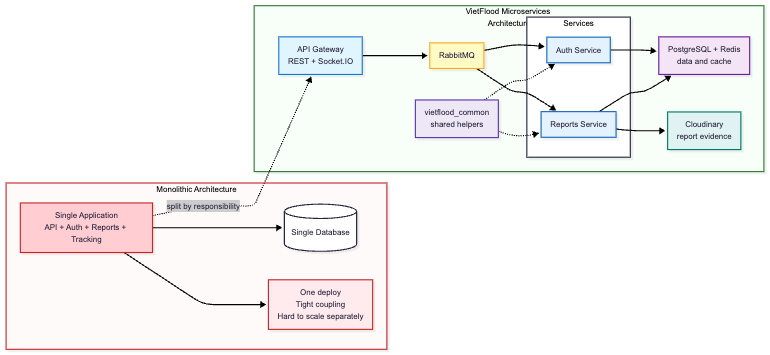
\includegraphics[width=0.9\linewidth,height=0.48\textheight,keepaspectratio]{images/figure2-2-microservices-comparison.png}
    }{
        \fbox{
            \begin{minipage}[c][5.2cm][c]{0.9\linewidth}
                \centering
                Placeholder for Figure 2.2\\[0.4cm]
                Suggested image: compare one monolithic backend with the VietFlood split of API gateway, auth service, reports service, RabbitMQ, Redis, PostgreSQL, and Cloudinary.\\[0.3cm]
                File name: \texttt{images/figure2-2-microservices-comparison.png}
            \end{minipage}
        }
    }
    \caption{Comparison between a monolithic backend and the VietFlood microservices structure.}
    \label{fig:chapter2-microservices-comparison}
\end{figure}

Figure~\ref{fig:chapter2-microservices-comparison} shows the difference between a single backend and the VietFlood structure. In VietFlood, the API gateway handles the public interface, the authentication service owns identity and tokens, and the reports service owns flood reports and evidence metadata. This division is not meant to make the prototype larger for its own sake. It is meant to keep the responsibilities visible.

\subsection{API Gateway Pattern}

The API gateway is the public entrance to the VietFlood backend. Mobile and web clients do not call the authentication service or reports service directly. They call the gateway, and the gateway forwards the request to the correct internal service. This follows the common gateway pattern, where a client-facing component hides internal service structure and provides one stable API surface \cite{bass2021softwareArchitecture,nestjsDocs}.

In VietFlood, the gateway handles authentication routes, report routes, multipart evidence upload, and Socket.IO tracking events. For report creation, it receives uploaded files through the \texttt{files} field, sends the file buffers to Cloudinary, and forwards the report payload and evidence metadata to the reports service. This keeps file upload concerns close to the public HTTP layer while keeping report persistence inside the reports service.

The gateway also hosts the live tracking entry point. A connected client can send a \texttt{send-location} event. The gateway checks latitude and longitude before broadcasting a \texttt{receive-location} event. Invalid payloads return \texttt{location-error}, and disconnected sockets are announced through \texttt{user-disconnected}. These events are small, but they show how real-time data can be added without changing the normal report API.

\subsection{Message Queues Between Services}

RabbitMQ is used for communication between the API gateway and internal backend services \cite{nestjsMicroservicesDocs,rabbitmqConfirmsDocs}. The gateway sends authentication-related messages to the auth queue and report-related messages to the reports queue. The corresponding service consumes the message, performs the work, and returns the result.

This design makes service boundaries clearer. For example, the gateway receives a sign-in request, but password checking and token creation belong to the authentication service. The gateway receives a create-report request, but report persistence belongs to the reports service. The gateway coordinates the request; it does not own all business logic.

Message-based communication also changes how errors are handled. A service may be unavailable or slow, so the gateway needs controlled timeouts and predictable responses. This is more work than a direct function call, but it reflects the realities of distributed systems and gives the project a useful technical foundation.

\subsection{Authentication and Role-Based Access}

VietFlood uses password-based authentication, JWT access tokens, refresh tokens, and role checks. Passwords are hashed with bcrypt before storage \cite{provos1999bcrypt}. After sign-in, the system returns an access token and refresh token. The access token follows the JWT model, where signed claims can be checked by protected routes \cite{jones2015jwt}.

The project uses three roles: citizen, relief, and admin. Citizens create reports and view reports linked to their own account. Relief users use mobile screens for broader report awareness and map-related viewing. Administrators use the web dashboard to inspect reports, update status, and manage users. This separation matters because report review and user management should not be available to every signed-in user.

The mobile application uses role-aware navigation so users see screens that match their role. The web dashboard checks the current profile before allowing admin pages to appear. The backend protects sensitive operations with authentication and role guards. Together, these layers keep access control from depending only on the user interface.

\subsection{Media Evidence and Cloud Storage}

Photo evidence can make a flood report easier to judge. A description can say that a street is flooded, but an image can show water level, road blockage, damage, or surrounding conditions. VietFlood stores uploaded evidence in Cloudinary instead of storing raw image files directly in PostgreSQL \cite{cloudinaryUploadDocs}.

The upload path begins at the API gateway. The gateway receives file buffers from the mobile app, uploads them to the \texttt{vietflood/reports} folder in Cloudinary, and passes the returned URL, public ID, and resource type to the reports service. The reports service stores this evidence metadata with the report. The URL supports preview and display. The public ID supports cleanup when a report is removed.

This design separates media storage from report storage. PostgreSQL keeps structured report data, while Cloudinary handles media files and delivery. Shared Cloudinary helpers in \texttt{vietflood\_common} keep upload and delete behavior reusable across services.

\begin{figure}[htbp]
    \centering
    \IfFileExists{images/evidence_flow.png}{
        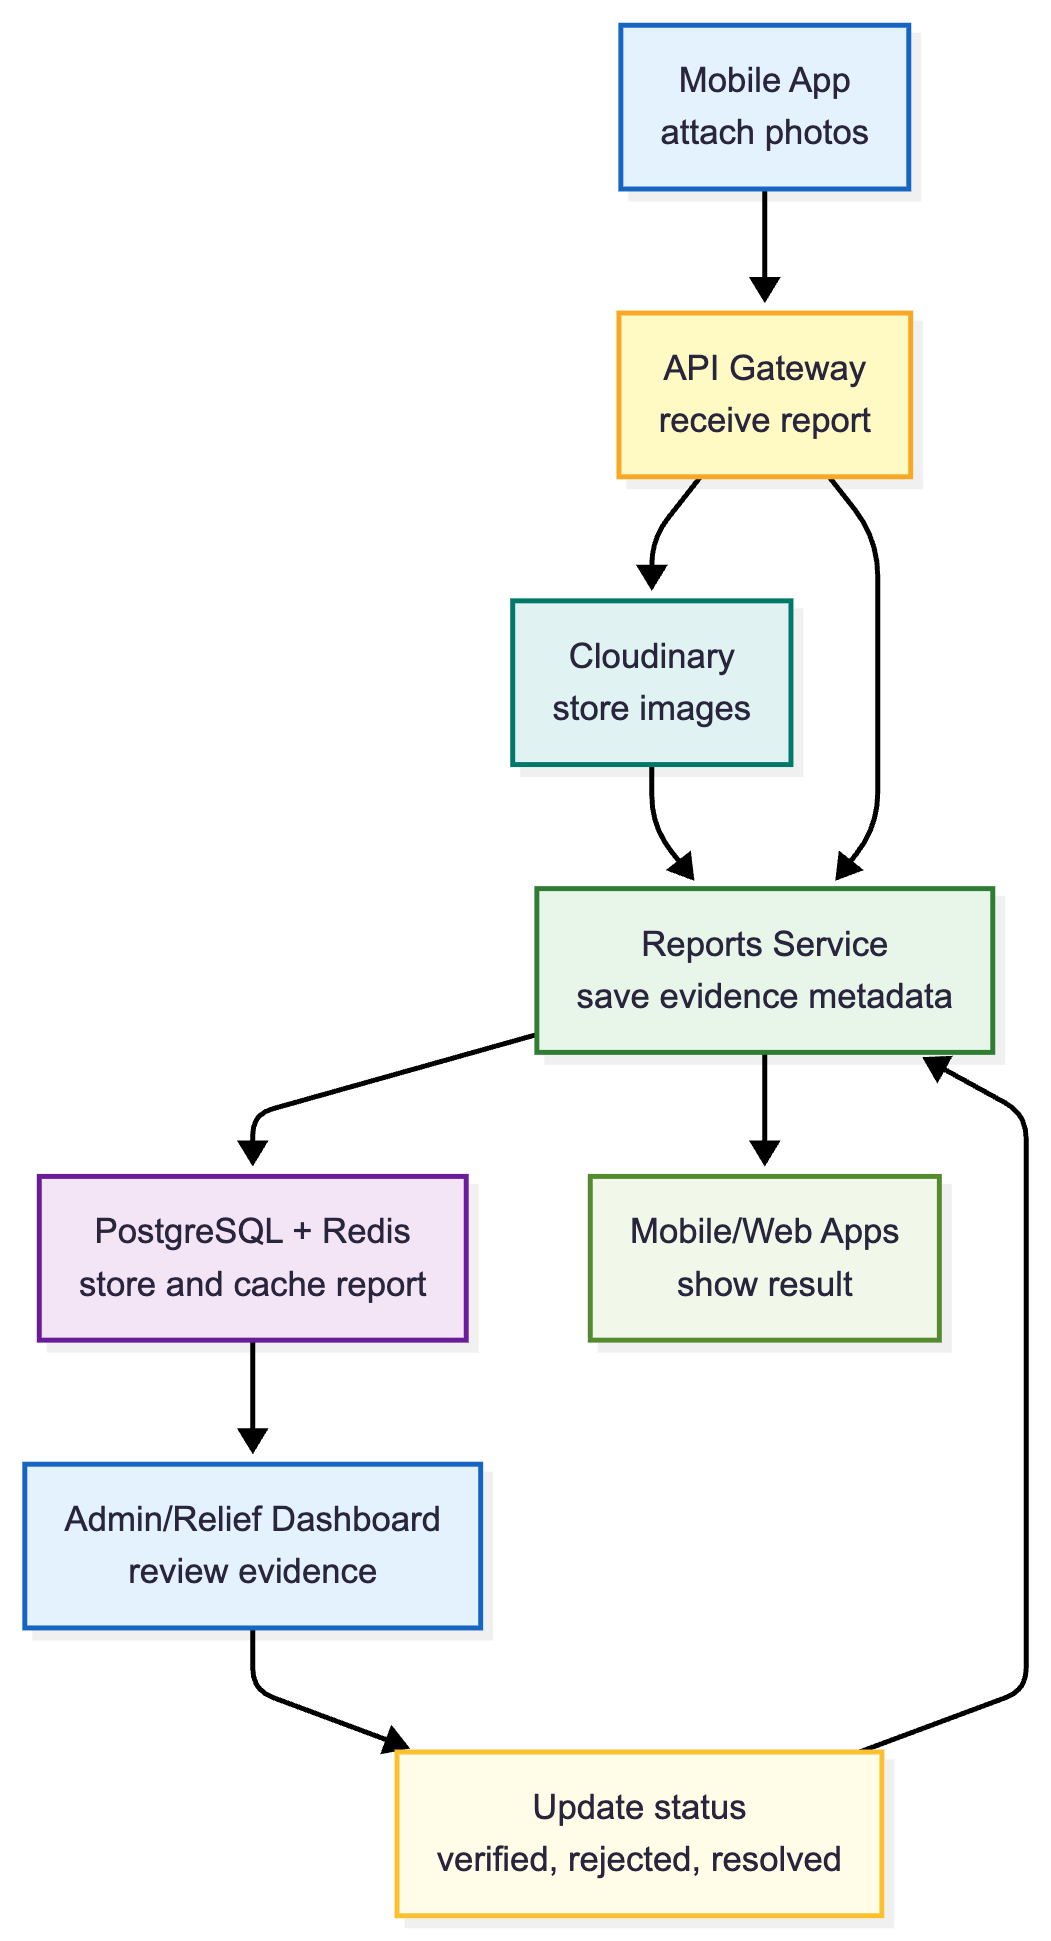
\includegraphics[width=0.88\linewidth,height=0.46\textheight,keepaspectratio]{images/evidence_flow.png}
    }{
        \fbox{
            \begin{minipage}[c][5cm][c]{0.88\linewidth}
                \centering
                Placeholder for Figure 2.3\\[0.4cm]
                Suggested image: mobile photo upload, API gateway, Cloudinary, reports service, PostgreSQL evidence metadata, and dashboard preview.\\[0.3cm]
                File name: \texttt{images/evidence\_flow.png}
            \end{minipage}
        }
    }
    \caption{Evidence upload and review flow in VietFlood.}
    \label{fig:chapter2-evidence-flow}
\end{figure}

Figure~\ref{fig:chapter2-evidence-flow} shows the technical path of evidence upload. The next figure pairs that system flow with screenshots from the actual application so the reader can connect the architecture to the user experience.

\begin{figure}[htbp]
    \centering
    \IfFileExists{images/figure2-4-mobile- evidence-upload.png.jpg}{
        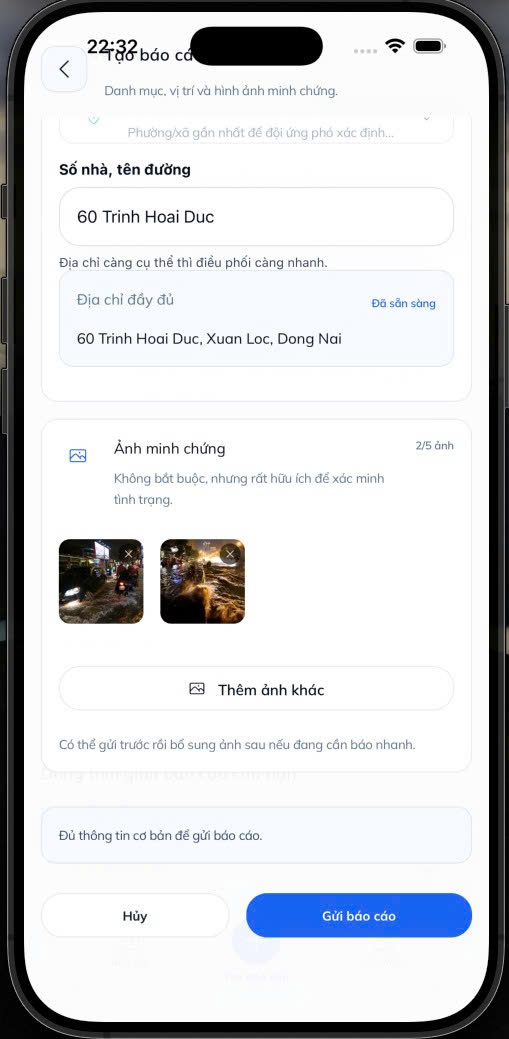
\includegraphics[width=0.38\linewidth,height=0.34\textheight,keepaspectratio]{images/figure2-4-mobile- evidence-upload.png.jpg}
    }{
        \fbox{
            \begin{minipage}[c][4.8cm][c]{0.38\linewidth}
                \centering
                Placeholder for mobile screenshot\\[0.35cm]
                Suggested image: report creation screen with attached photo evidence.\\[0.25cm]
                File name:\\
                \texttt{figure2-4-mobile-}\\
                \texttt{evidence-upload.png.jpg}
            \end{minipage}
        }
    }
    \hspace{0.03\linewidth}
    \IfFileExists{images/figure2-4-dashboard-relief-evidence-review.jpg}{
        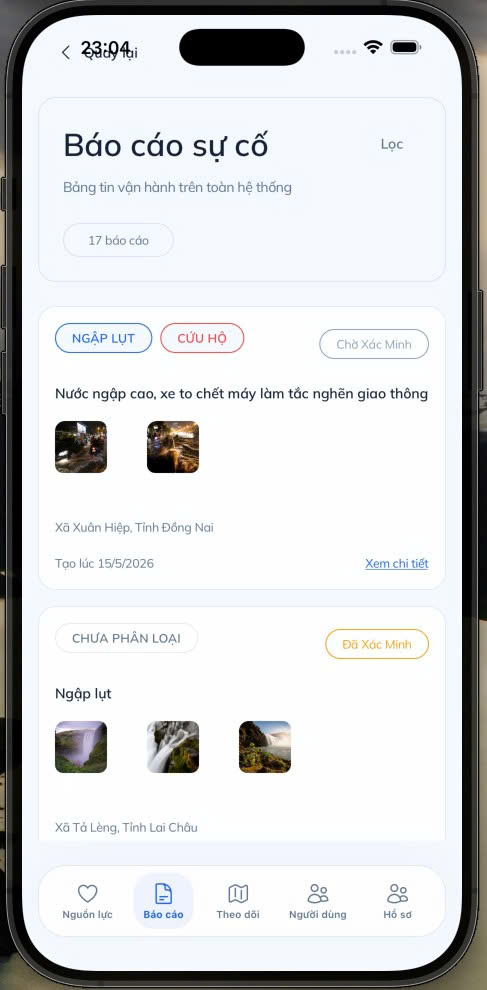
\includegraphics[width=0.52\linewidth,height=0.34\textheight,keepaspectratio]{images/figure2-4-dashboard-relief-evidence-review.jpg}
    }{
        \fbox{
            \begin{minipage}[c][4.8cm][c]{0.52\linewidth}
                \centering
                Placeholder for dashboard screenshot\\[0.35cm]
                Suggested image: dashboard showing evidence preview and report details.\\[0.25cm]
                File name:\\
                \texttt{figure2-4-dashboard-relief-}\\
                \texttt{evidence-review.jpg}
            \end{minipage}
        }
    }
    \caption{Mobile evidence upload and dashboard evidence review in VietFlood.}
    \label{fig:chapter2-evidence-screenshots}
\end{figure}

\subsection{Database and Cache}

PostgreSQL is the main persistent database for VietFlood. The backend uses TypeORM to map application entities to database tables \cite{typeormDocs}. Reports store both ordinary relational fields, such as status and coordinates, and JSON evidence metadata. PostgreSQL supports JSON data when flexible structured fields are needed inside a relational database \cite{postgresqlJsonDocs}.

Redis is used as a focused cache rather than a replacement for the database \cite{redisDocs}. The reports service can cache report lookup data and clear stale entries when a report changes. PostgreSQL remains the source of truth, while Redis helps reduce repeated reads for data that may be requested multiple times.

The cache scope is deliberately limited. A broad cache layer can become difficult to reason about if invalidation is unclear. VietFlood uses caching where the key pattern and update behavior are understandable, which fits the size of the prototype.

\subsection{Shared Infrastructure Package}

The backend services reuse common infrastructure through the \texttt{vietflood\_common} package. This package exports the Redis module and service, Cloudinary module and service, and a structured logger. The logger can include timestamp, log level, service name, trace context, user ID, role, request path, and HTTP method when that context is available.

The shared package reduces repeated code across the gateway, authentication service, and reports service. More importantly, it keeps infrastructure behavior consistent. A Redis connection should be configured the same way across services. A Cloudinary upload should return evidence metadata in the same shape. A log message should carry enough context to trace work through the backend.

\subsection{Containerized Deployment}

VietFlood uses Docker Compose to run the backend services together with Redis and RabbitMQ \cite{dockerComposeDocs}. The local setup builds service images from the repository, while the production-oriented configuration uses Docker Hub images for the gateway, auth service, and reports service. Environment variables provide database URLs, Redis settings, RabbitMQ credentials, JWT secrets, refresh-token secrets, Cloudinary credentials, and admin seed values.

The project also includes a GitHub Actions deployment workflow. The workflow builds service images, tags them, pushes them to Docker Hub, configures Azure App Service, and restarts the deployed application \cite{githubActionsDocs,azureAppServiceContainersDocs}. This is aligned with continuous delivery practices, where builds and deployments should be repeatable instead of depending on manual steps \cite{humble2010continuousDelivery,kim2016devopsHandbook}.

\section{Comparison of Design Approaches}

VietFlood can be compared with two simpler approaches. The first is informal reporting through chat, phone calls, and social media. This is fast and familiar, but it does not produce a searchable report database or a clear status history. The second is a single-server reporting website. This is easier to develop, but authentication, reports, evidence, caching, and live tracking can become tightly connected as the project grows.

The VietFlood approach sits between those two options. It is more structured than informal reporting and more modular than a single backend, but it is still small enough to explain clearly. The API gateway owns the public interface. The authentication service owns accounts and tokens. The reports service owns flood report data and evidence metadata. Redis, PostgreSQL, RabbitMQ, Cloudinary, and Socket.IO each support a specific infrastructure need.

This design adds engineering effort. There are more services to configure, more environment variables to manage, and more failure points to consider. The benefit is that each responsibility is visible. For a thesis prototype, that tradeoff is useful because it demonstrates not only a working application, but also the architectural reasoning behind the application.
